%\chapter{Biologischer Hintergrund}\label{chap:biology}

%In diesem Kapitel wird beschrieben, in welchem Zusammenhang der Chlorophyllgehalt einer Pflanze mit der Vitalität eben dieser steht. Und es wird erklärt wie der Chlorophyllgehalt %genutzt werden kann, um  den Stresslevel einer Pflanze zu bestimmen.

\chapter{Konzept}\label{chap:concept}

\section{Normalized Difference Vegetation Index}\label{sec:ndvi}

Es gibt eine starke Korrelation zwischen dem physiologischen Status einer Pflanze und deren Chlorophyllgehalt. Faktoren wie Krankheit, Dürre oder Umweltverschmutzung haben einen negativen Einfluss auf den Chlorophyllspiegel.\cite{ref:hendry} Messungen haben ergeben, dass es einen Verbindung zwischen dem Reflexionsgrad im nahen Infrarotbereich und im Rotbereich und dem Chlorophyllgehalt gibt. Das heißt, dass eine gesunde, adulte Pflanze im nahen Infrarotbereich stärker reflektiert als zum Beispiel eine pathologisch veränderte Pflanze. Jedoch bleibt die Reflexion im roten Lichtspektrum in beiden Fällen vergleichsweise schwach. Andere vegetationsfreie Oberflächen wie Acker, Straßen oder Wasser strahlen auch im nahen Infrarotbereich schwach zurück. Dadurch ergibt sich eine zerstörungsfreie Methode, mit einer Multispektralkamera die Vitalität ("`Grünheit"') einer oder mehrerer Pflanzen zu bestimmen.\cite{ref:anatoly} \\\\
Eine multispektralen Aufnahme kann mithilfe der Formel 
\begin{equation}\label{equation:ndvi}
	NDVI = \frac{Band_{NIR} - Band_{Red}} {Band_{NIR} + Band_{Red}}
\end{equation}
dazu genutzt werden, den \textit{Normalized Difference Vegetation Index} (NDVI) zu berechnen. Wobei $Band_{NIR}$ der nahe Infrarotbereich (Near Infrared) und $Band_{RED}$ der sichtbare rote Bereich des elektromagnetischen Spektrums ist. Der NDVI gibt quantifizierte Werte im Bereich von $-1$ bis $1$ zurück. Dabei deuten Werte, die kleiner als $0$ sind, auf Wasserobflächen hin. $0$ bedeutet keine Vegetation. Bei Werte nahe $0$ handelt es sich um spärliche oder ungesunde Vegetation. Das bedeutet je näher ein Wert an $1$ ist, desto dichter bewachsen und gesünder ist die beobachtete Vegetationsfläche.\cite{ref:nasa} Dass bei einem niedrigen, positiven NDVI nicht unterschieden werden kann, ob eine Fläche kaum bewachsen ist oder ungesunde Vegetation besitzt, kann hier vernachlässigt werden. Das Gebiet, das in dieser Arbeit untersucht wird, ist ein bewachsenes Feld, so kann man geringe Vegetation ausschließen. 

\section{Sentinel-2}\label{sec:sentinel2}

Die Sentinel-2-Satelliten sind eine von sechs Satellitenarten (Sentinel-1 bis -6) des Copernicus-Programms\footnote{Das Copernicus-Programm wurde von der Europäischen Union zur Erdbeobachtung ins Leben gerufen. Die gesammelten Daten werden für wissenschaftliche, wirtschaftliche und private Anwendungszwecke zur Verfügung gestellt.\cite{ref:copernicus}}, die zur Erdbeobachtung in einen 786 km hohen sonnensynchronen Orbit gebracht wurden. Die Instrumente der Sentinel-2-Satelliten können Aufnahmen in Bereichen des roten und nahen Infrarot- bis hin zum Kurzwelleninfrarotspektrums. Die Aufnahmen haben Gesamtgröße von $100*100$ km und je nach Band eine von Auflösung von 10m, 20m oder 60m (s. Tabelle \ref{tab:resolutions}).

\begin{table}[h]
\begin{tabular}{c|c|c|c}
Bandnummer & Räumliche Auflösung & Mittlere Wellenlänge (nm) & Bandbreite (nm) \\
\hline
B1 & 60 & 443,9 & 27\\
B2 & 10 & 496,6 & 98\\
B3 & 10 & 560 & 45\\
B4 & 10 & 664,5 & 38\\
B5 & 20 & 703,9 & 19\\
B6 & 20 & 740,2 & 18\\
B7 & 20 & 782,5 & 28\\
B8 & 10 & 835,1 & 145\\
B8a & 20 & 864,8 & 33\\
B9 & 60 & 945 & 26\\
B10 & 60 & 1373,5 & 75\\
B11 & 20 & 1613,7 & 143\\
B12 & 20 & 2202,4 & 242\\
\end{tabular}
\caption{Räumliche und spektrale Auflösungen von Sentinel-2A\cite{ref:sentinel:radiores}}\label{tab:resolutions}
\end{table}
\noindent
Besonders wichtig sind die Bänder B4 (Rot) und B8 (Nahes Infrarot). Mit diesen Bändern kann der NDVI (s. Kapitel \ref{sec:ndvi}) berechnet werden.\cite{ref:sentinel:ndvi} Die Sentinel-2-Satelliten bieten mit $10*10$ m pro Pixel eine hohe räumliche Auflösung.\footnote{Im Vergleich hat zum Beispiel der Landsat-8-Satellit, dessen Daten ebenfalls frei verfügbar sind, eine relativ geringe Auflösung von $30*30$ m.} Diese Eigenschaft ist wichtig, um eine mögliche Infizierung genau eingrenzen zu können.\\\\
Dabei ist es auch wichtig, dass die Satelliten regelmäßige Daten liefern können. Durch die gemeinsame Konstellation übertragen die Plattformen alle fünf Tage Daten über einen spezifischen Punkt auf der Erdoberfläche.\cite{ref:sentinel:resolutions} Damit ist gewährleistet, dass der Feldbesitzer ohne persönliche Inspektion ein bis zweimal in der Woche eine Gesundheitseinschätzung über seine Felder erhält.

\section{Mask R-CNN}\label{sec:maskrcnn}
In Kapitel \ref{sec:ndvi} und \ref{sec:sentinel2} wurde erklärt wie Daten über die möglichen Erkrankungen geliefert und verarbeitet werden können. Auf den zugrunde liegenden Bilddaten soll nun ein künstliches neuronales Netzwerk (KNN) trainiert werden. In diesem Kapitel wird darauf eingegangen, welche Anforderungen an das KNN gestellt werden und warum das Titel gebende Netz ausgewählt wurde.

\subsection{Grundlagen}\label{sec:sub:basics}

\begin{figure}[ht]
  \centering
  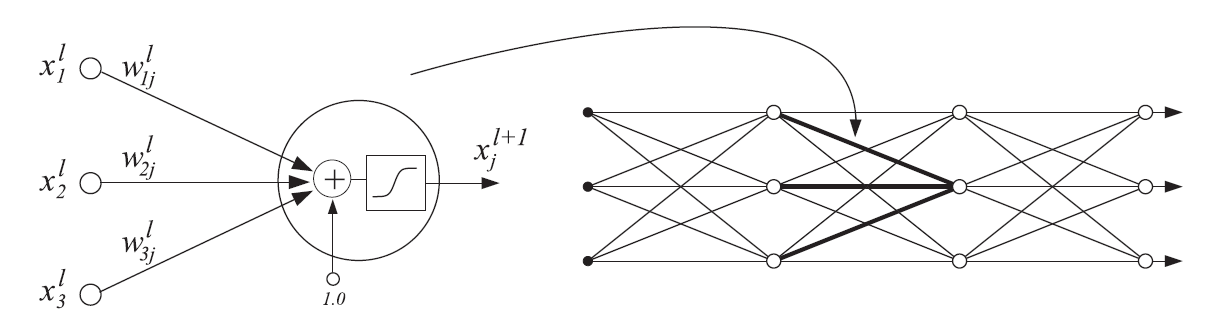
\includegraphics[width=0.95\textwidth]{pics/neural-net.PNG}
  \caption[Künstliches neuronales Netz]{Künstliches neuronales Netz\cite{ref:verrelst}}
  \label{fig:instance-segmentation}
\end{figure}

\noindent
Künstliche neuronale Netze sind nach dem Vorbild von biologischen neuronalen Netzen gebildet worden. So ist ein KNN ebenfalls eine Verbindung von künstlichen Neuronen. Diese Neuronen sind in Schichten angeordnet und jede die Neuronen einer Schicht sind mit den Neuronen nächsten bzw. letzten Schicht verbunden. Ein Neuron besitzt mehrere Eingangsverbindungen (Gewichte) und ein Ausgangsneuron. Ob ein Neuron "`feuert"', wird durch eine lineare oder nicht-lineare Aktivierungsfunktion bestimmt. Die Eingangsgewichte sind veränderbare Werte, die je nach Höhe einen starken oder niedrigen Einfluss auf die Aktivierungsfunktion haben.
\begin{equation}\label{equ:neuron}
x^{l+1}_{j}=f(\sum\nolimits_i w^l_{ij}x^l_i + w^l_{bj})
\end{equation}
beschreibt das Neuron $j$ in Schicht $l+1$, wobei
\begin{itemize}
	\item $w^l_{ij}$ die Gewichte sind, die Neuron $i$ in Schicht $l$ mit Neuron $j$ verbinden.
	\item $w^l_{bj}$ der Biasterm des $j$-ten Neurons in Schicht $l$ ist.
	\item $f$ die Aktivierungsfunktion ist.\cite{ref:verrelst}
\end{itemize} 

\todo{Hier sollte ggf. noch die Erklärung von Training und Validierung hin. Oder doch eigenes Kapitel in overfitting?}
\noindent
Es gibt noch andere Arten von KNNs. Die Arten, die Teil dieser Arbeit sind, werden in den folgenden Kapitel beschrieben.

\subsection{Anforderungen}\label{sec:sub:requirements}
Das KNN muss in der Lage sein, wahrscheinliche Krankheiten in der zu untersuchenden Agrarfläche möglichst genau eingrenzen und klassifizieren zu können. Das ist besonders wichtig, wenn ein Feld von multiplen Krankheiten betroffen ist.\\\\
Es ist damit zu rechnen, dass Daten unter bewölkten Bedingungen aufgenommen werden. Nach starken Niederschlägen können Acker teils oder gänzlich überflutet sein.\cite{ref:root-rot} Das sorgt selbst unter wolkenfreien Bedingungen für einen niedrigen NDVI, obwohl die Nutzpflanzen gesund sind. Das neuronale Netz muss mit solchen \glqq Ausreißern\grqq{} umgehen können.
\\\\
Daraus ergeben sich folgende Kriterien für das neuronale Netzwerk:

\begin{itemize}
	\item Erkennung auf Pixelebene
	\item Robustheit
	\item Schnelles Training
	\item Hohe Genauigkeit 
\end{itemize}

\subsection{Mask R-CNN}\label{sec:sub:mask-rcnn}

\begin{figure}[ht]
  \centering
  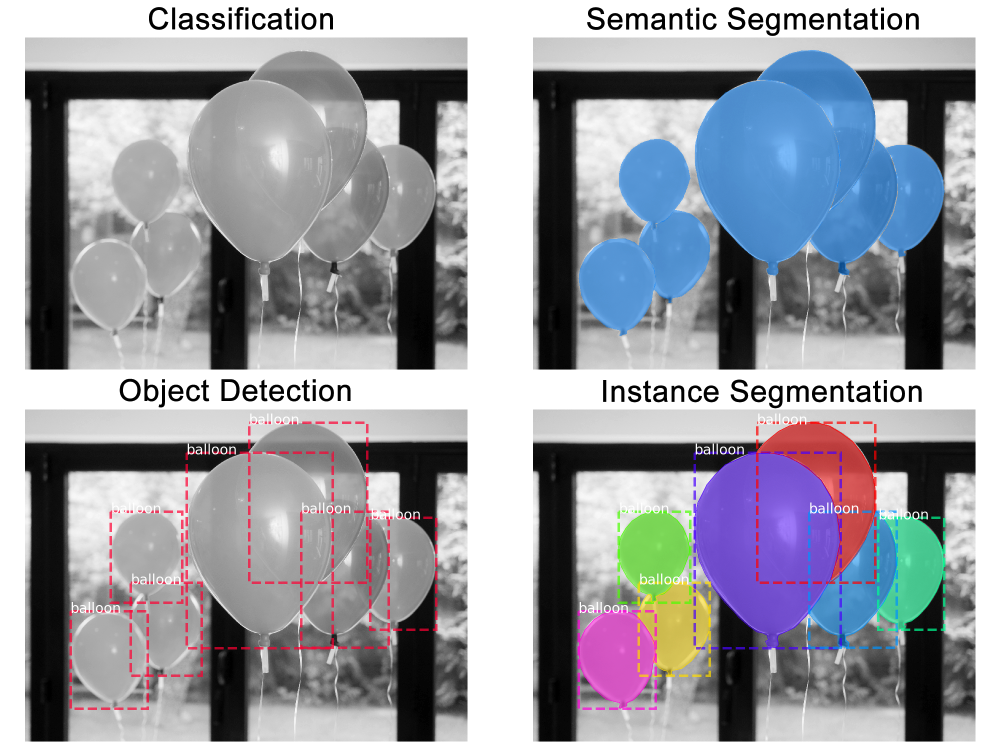
\includegraphics[width=0.95\textwidth]{pics/instance-segmentation.png}
  \caption[Instanzsegmentierung]{Unterschied Klassifizierung / semantische Segmentierung / Objekterkennung / Instanzsegmentierung\cite{ref:matterport:maskrcnn}}
  \label{fig:instance-segmentation}
\end{figure}

Einfache Klassifizierung (engl.: classification) ordnet Bilder als Ganzes einer Klasse zu. \textit{Semantische Segmentierung} (engl.: semantic segmentation) beschreibt die Klassifizierung auf Pixelebene. Es wird erkannt zu welcher Klasse eine Menge von Pixeln gehören, aber es wird nicht zwischen einzelnen Objekten unterschieden. \textit{Objekterkennung} (engl.: object detection) entdeckt und lokalisiert unterschiedliche Objekte, indem es eine Bounding Box um jedes erkannte Objekt zieht. Jedoch fehlt hier die pixelgenaue Abgrenzung einzelner Objektinstanzen. \text{Instanzsegmentierung} (engl.: instance segmentation) kombiniert \textit{Objekterkennung} und \textit{semantische Segmentierung} und ist so in der Lage zwischen einzelnen Objekten zu unterscheiden und ihnen entsprechende Pixel zuzuordnen (s. Abb. \ref{fig:instance-segmentation}).\cite{ref:maskrcnn}
\\\\
